\section{Development}

\subsection{Problem scope and chosen election datasets}
Portuguese local election results are distributed as 
multi-sheet CNE workbooks. Lists are often 
identified by local codes (e.g. A, B in Lisboa 2021), 
not only national party acronyms. Vote counts, turnout,
 and mandates appear in different sheets; boundary files 
 use another naming scheme. 
 The project goal is a database-centred application: store data in a normalized schema and a warehouse, 
 load it through a rerunnable ETL, expose non-trivial SQL 
 (D'Hondt, window functions, ROLLUP, CUBE), and 
 serve a thin web UI, in this case using Flask, that queries PostgreSQL with psycopg2 (no ORM).   \\
 So, for this project, we chose to focus on the 2021 and 2017 local elections. 
 \begin{itemize}
        \item \textbf{2021 Local Elections:} This dataset includes detailed results from the 2021 local elections in Portugal, covering various municipalities and parties. It provides a comprehensive view of the electoral landscape during that period.
        \item \textbf{2017 Local Elections:} This dataset contains results from the 2017 local elections, allowing us to analyze trends and changes in voter behavior and party performance over time.
        \item \textbf{DGT CAOP 2021:} This dataset includes boundary files for the municipalities, which are essential for spatial analysis and visualization of election results.
\end{itemize}
\subsection{Operational Schema and Warehouse Design Rationale}
The system uses three PostgreSQL schemas: staging 
(\texttt{sql/05_staging_schema.sql}), operational (\texttt{sql/01_operational_schema.sql}),
 and warehouse (\texttt{sql/02_warehouse_schema.sql}).  \\
The following ER diagrams (obtained with pgAdmin's ERD tool) illustrate the design of the operational and warehouse schemas, 
highlighting the relationships between tables and the overall structure of the database. The operational schema is designed to store raw and processed data for day-to-day operations, while the warehouse schema is optimized for analytical queries and reporting.

\textbf{Keys and indexing.} Primary and foreign keys enforce election--organ--territory--party integrity; \texttt{candidacy} is the hub linking lists to \texttt{vote\_result}, \texttt{seat\_result}, and related facts. B-tree indexes on \texttt{candidacy} (election, organ, municipality) and on \texttt{vote\_result} (candidacy, votes descending) match the usual filters (one contest per municipality, top parties by votes). GiST indexes on district and municipality \texttt{geometry} support map bounding-box queries. Warehouse indexes on fact and dimension keys speed star-schema joins; \texttt{party\_municipality\_summary} is indexed by election, municipality, and party for quick lookups after \texttt{refresh\_party\_municipality\_summary()}.

\begin{figure}[h!]
    \begin{center}
    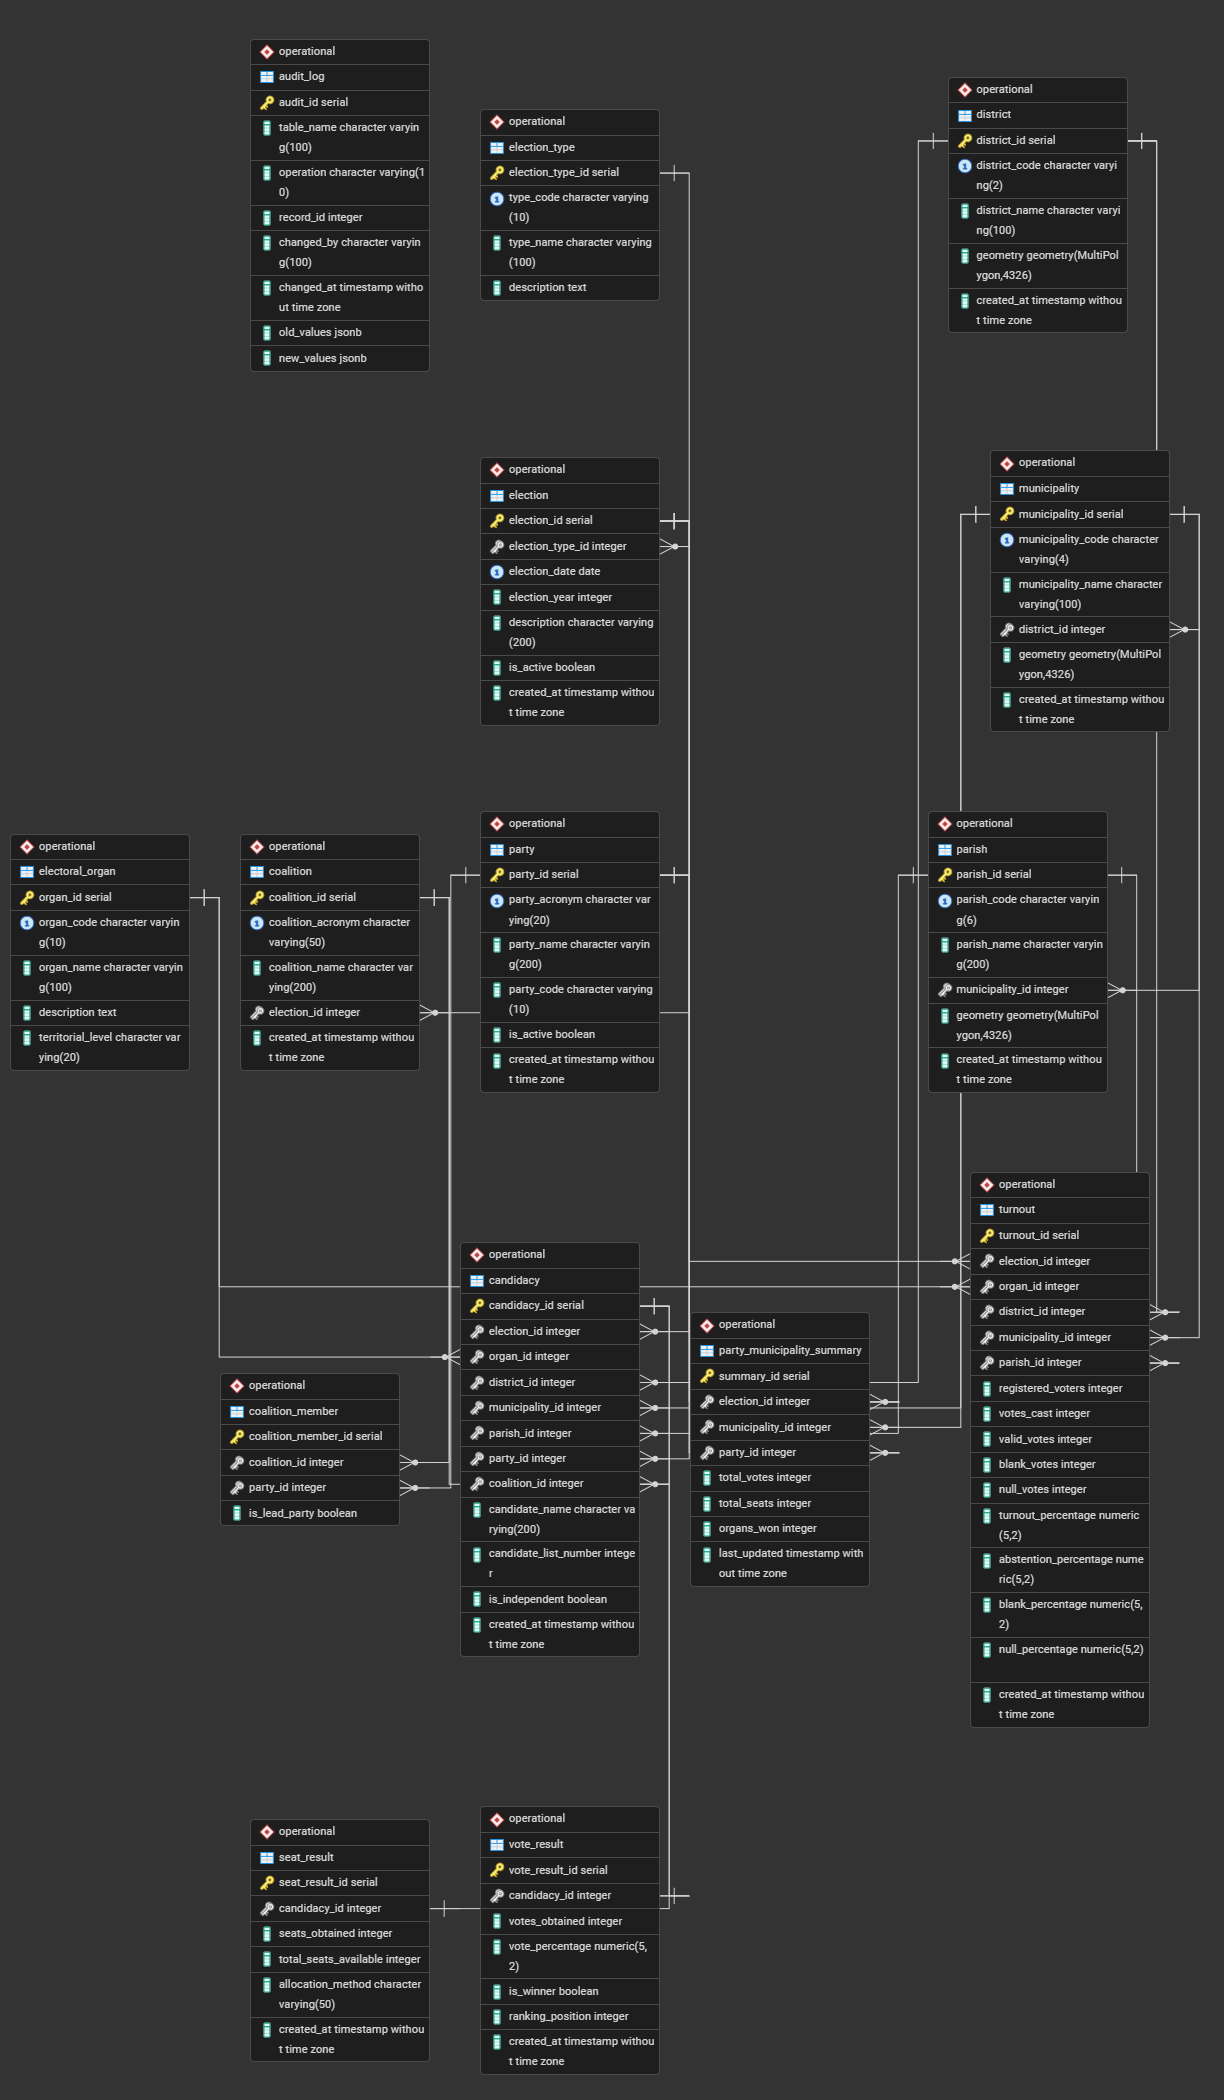
\includegraphics[width=10cm, height=9cm]{../er_diagrams/operational_schema_er.png}
    \caption{Operational Schema ER Diagram}
    \end{center}
\end{figure}

\begin{figure}[h!]
    \begin{center}
    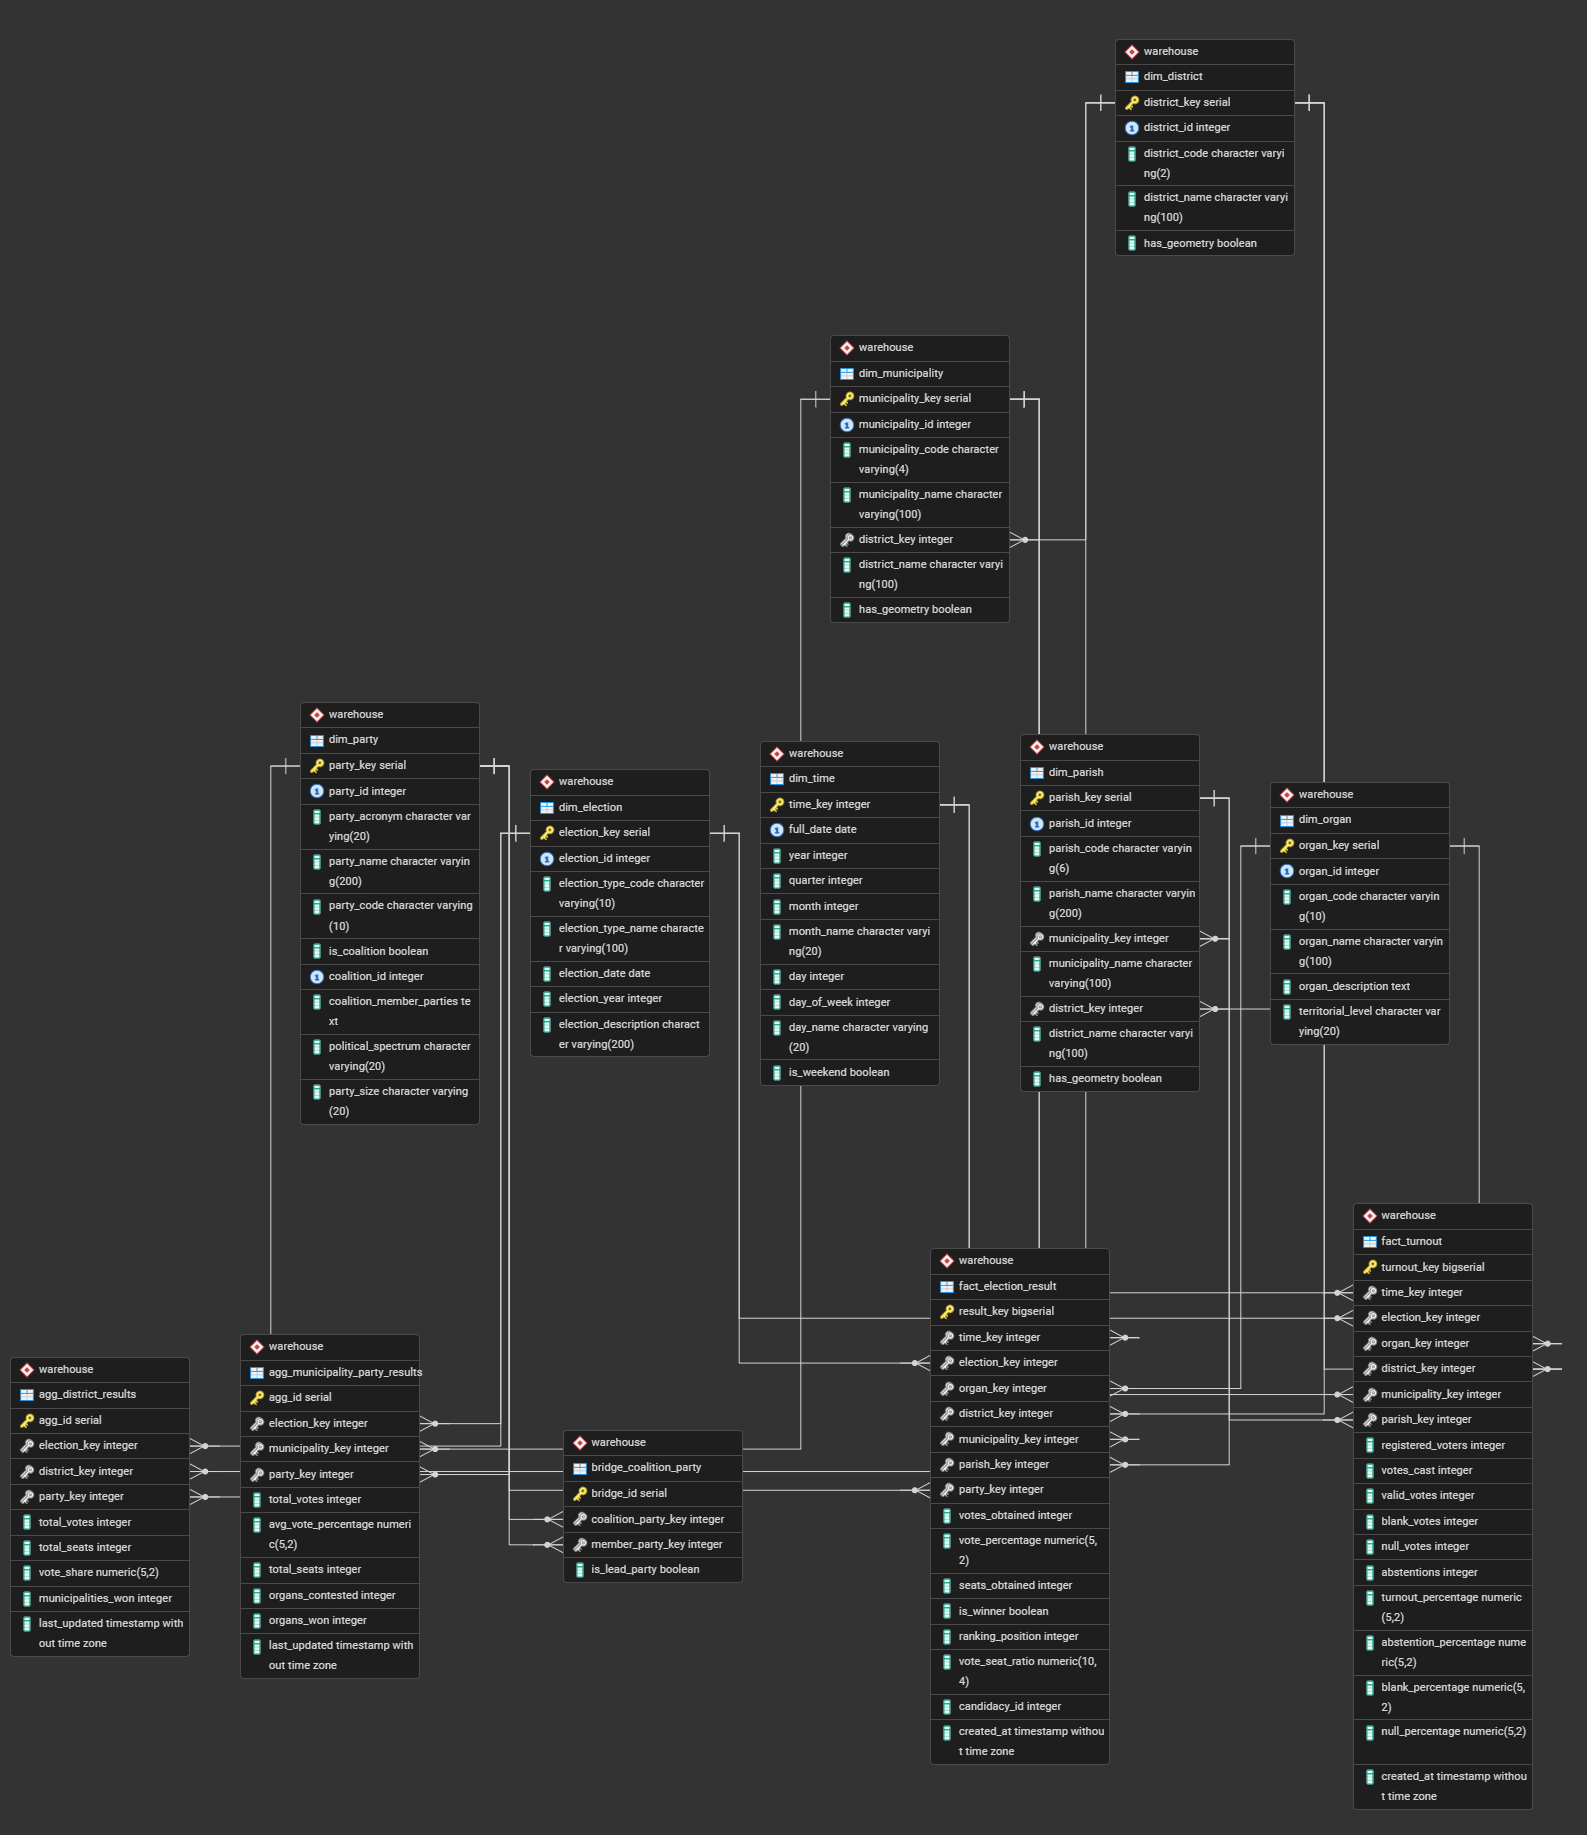
\includegraphics[width=10cm, height=9cm]{../er_diagrams/warehouse_star_schema.png}
    \caption{Warehouse Star Schema ER Diagram}
    \end{center}
\end{figure}


\subsection{ETL Pipeline}
The Python ETL (\texttt{etl/run\_etl.py}, \texttt{--mode full}) loads \textbf{Câmara Municipal (CM)} results at \textbf{municipality} level for elections \texttt{aut\_2017} and \texttt{aut\_2021}. Votes and turnout come from CNE \textbf{mapa\_1} (wide Excel, unpivoted in \texttt{pipeline/extract.py} into \texttt{staging.stg\_election\_results} and \texttt{stg\_turnout\_data}); official seat counts from \textbf{mapa\_2} (\texttt{pipeline/load\_seats.py} $\rightarrow$ \texttt{seat\_result}). District and municipality boundaries are joined from DGT CAOP via \texttt{pipeline/transform\_geo.py}. Each run is logged in \texttt{staging.stg\_etl\_run\_log} and can be repeated per \texttt{election\_id}.

\begin{center}
\small
\begin{tabular}{|l|l|l|}
\hline
\textbf{Phase} & \textbf{Module} & \textbf{Main output} \\
\hline
Extract & \texttt{extract.py} & \texttt{stg\_election\_results}, \texttt{stg\_turnout\_data} \\
Operational & \texttt{transform\_operational.py} & parties, \texttt{candidacy}, \texttt{vote\_result}, \texttt{turnout} \\
Geometries & \texttt{transform\_geo.py} & PostGIS \texttt{geometry} on districts/municipalities \\
Warehouse & \texttt{load\_warehouse.py} & \texttt{dim\_*}, \texttt{fact\_*} \\
Seats & \texttt{load\_seats.py} & \texttt{seat\_result} (CNE mandates) \\
Post-load & \texttt{post\_load.py} & \texttt{party\_municipality\_summary}, turnout \% \\
\hline
\end{tabular}
\end{center}

\textbf{Cleaning and load policy.} Wide sheets are unpivoted to one row per list column; votes are coerced to integers; territory names are normalized (title case); only CM rows are kept (empty parish field). Parties are resolved with \texttt{get\_or\_create\_party}. Municipalities are matched to CAOP by \textbf{CNE names}, not a single official concelho code end-to-end. During bulk insert, \texttt{session\_replication\_role = replica} disables audit triggers; vote and turnout percentages are recomputed in post-load (\texttt{calculate\_turnout\_percentages}, \texttt{refresh\_party\_municipality\_summary}).

\textbf{Validation.} Spot checks for Lisboa, Porto, and Barrancos (2021) show zero mismatches against CNE for votes, turnout, percentages, and seats. About 50 municipalities appear in \texttt{mapa\_2} without corresponding \texttt{mapa\_1} rows; they remain without vote facts in the database (documented source gap, not an ETL bug).

\subsection{Functions, Views, and Triggers}
All functions, views, and triggers were implemented in PostgreSQL using PL/pgSQL.
\begin{itemize}
    \item \textbf{Functions:}
    \begin{itemize}
        \item \texttt{calculate_vote_percentage (p_candidacy_id)}: Calculate vote percentage for a candidacy.
        \item \texttt{get_party_performance_in_municipality (p_election_id, p_municipality_id,
        p_party_acronym)}: Get the performance of a party in a specific municipality.
        \item \texttt{get_top_parties (p_election_id, p_municipality_id, 
        p_organ_id, p_limit)}: Get the top parties in a specific municipality.
        \item \texttt{allocate_seats_dhondt (p_election_id, p_organ_id, 
        p_municipality_id, p_total_seats)}: Allocate seats based on the D'Hondt method for a specific election and municipality.
        \item \texttt{calculate\_turnout\_percentages ()}: Batch recompute turnout and related percentages after ETL.
        \item \texttt{get_or_create_party (p_party_acronym, p_party_name)}: 
        Get or create a party based on its acronym and name.
    \end{itemize}
    \item \textbf{Views:}
    \begin{itemize}
        \item \texttt{vw_complete_results}: A view that provides complete election results, including vote counts, percentages, and seat allocations for each candidacy.
        \item \texttt{vw_turnout_analysis}: A view that provides turnout analysis for each election and municipality.
        \item \texttt{vw_candidacy_details}: A view that provides complete candidacy information, including vote percentages and seat allocations.
        \item \texttt{vw_municipality_summary}: A view that summarizes election results by municipality, including total votes, turnout, and seat allocations.
        \item \texttt{vw_stg_missing_data}: A view that identifies any missing data in the staging tables, such as missing votes or candidacy information.
        \item \texttt{vw_stg_potential_duplicates}: A view that identifies potential duplicate records in the staging tables, such as duplicate votes or candidacies.
    \end{itemize}
    \item \textbf{Triggers:}
    \begin{itemize}
        \item \texttt{trg\_turnout\_percentages} (on \texttt{turnout}): before insert/update, derives turnout, abstention, blank, and null percentages from registered voters and votes cast.
        \item \texttt{trg\_vote\_percentages} (on \texttt{vote\_result}): before insert/update, sets \texttt{vote\_percentage} from the contest valid-vote total in \texttt{turnout}.
        \item \texttt{trg\_audit\_candidacy} and \texttt{trg\_audit\_vote\_result}: after changes on candidacy or vote rows, append rows to \texttt{audit\_log} via \texttt{trg\_audit\_log()}. Bulk ETL disables triggers; percentages and summaries are refreshed in post-load.
    \end{itemize}
\end{itemize}
\subsection{Analytical Queries}
Beyond operational functions and triggers, we added eight analytical views and \texttt{demonstrate\_dhondt} in \texttt{sql/04\_analytical\_queries.sql}. They are applied \textbf{after} ETL (not part of the load). The Flask UI does \textbf{not} query these objects: pages and APIs use operational tables and simpler warehouse/operational views (\texttt{vw\_candidacy\_details}, \texttt{vw\_municipality\_summary}, map endpoints) for municipality-level browsing, maps, and 2017 vs 2021 charts. Results from \texttt{ROLLUP}, \texttt{CUBE}, and district-wide ranking views are wide, hierarchical tables that would need separate report-style screens or exports; we kept them in PostgreSQL to satisfy the advanced SQL requirements and document findings without extending the web layer. They are meant for direct use in \texttt{psql}/pgAdmin or via \texttt{scripts/run\_sql\_demos.py}, which writes \texttt{docs/sql\_outputs/demo\_results.txt}.

\begin{center}
\small
\begin{tabular}{|l|l|}
\hline
\textbf{View / function} & \textbf{SQL technique} \\
\hline
\texttt{analytical\_query\_1\_party\_rankings} & \texttt{RANK}, running totals \\
\texttt{analytical\_query\_2\_district\_comparison} & Party \% vs district average \\
\texttt{analytical\_query\_3\_turnout\_analysis} & \texttt{NTILE}, quartiles \\
\texttt{analytical\_query\_4\_rollup\_hierarchical} & \texttt{GROUP BY ROLLUP} \\
\texttt{analytical\_query\_5\_cube\_multidimensional} & \texttt{GROUP BY CUBE} \\
\texttt{analytical\_query\_6\_advanced\_aggregates} & \texttt{FILTER}, \texttt{STRING\_AGG}, \texttt{ARRAY\_AGG} \\
\texttt{analytical\_query\_8\_cross\_district\_comparison} & Cross-district ranks \\
\texttt{demonstrate\_dhondt} & Ranked D'Hondt quotients \\
\hline
\end{tabular}
\end{center}

\textbf{Key findings (CM, validated against CNE samples).}
\begin{itemize}
    \item \textbf{Lisboa 2021:} lists \textbf{A} (35.35\%) and \textbf{B} (34.38\%) lead; local codes matter more than a single national-party label (\texttt{calculate\_vote\_percentage} matches stored \%).
    \item \textbf{Cross-year Lisboa:} 2017 winner \textbf{PS} (43.89\%) vs 2021 winner \textbf{A} (35.35\%) --- same municipality, different list coding between elections.
    \item \textbf{District contrast (2021):} Lisboa list A is +14.87 percentage points above its district average; PSD is $-$20.74 pp (\texttt{analytical\_query\_2}).
    \item \textbf{Seats:} CNE \texttt{mapa\_2} gives A/B seven mandates each in a 17-seat council; \texttt{allocate\_seats\_dhondt} with \textbf{7} seats is an illustrative run (3+3+1), separate from official allocation.
    \item \textbf{Porto D'Hondt (7 seats):} PS 5, B 2 (\texttt{demonstrate\_dhondt}, \texttt{run\_sql\_demos.py}).
    \item \textbf{Warehouse scale:} after full load, $\sim$1\,256 \texttt{fact\_election\_result} and $\sim$281 \texttt{fact\_turnout} rows (see demo output tail).
\end{itemize}

\subsection{Frontend Overview}
The web client (\texttt{app/app.py}) is a thin \textbf{Flask} application that queries PostgreSQL with \textbf{psycopg2} and raw SQL---no ORM. The user selects an election year from the navbar (\texttt{election\_id} query parameter); all pages and chart APIs scope results to that election.

\textbf{Pages and data flow.} \texttt{/} shows national summary statistics and a Leaflet map of districts (GeoJSON from \texttt{/api/map/districts}; click opens \texttt{/district/<id>}). The districts page lists all concelhos with average turnout and a comparison chart. \texttt{/municipality/<id>} renders CM results as an HTML table plus Chart.js bar charts (\texttt{/api/charts/party\_comparison}). \texttt{/analytics} compares \textbf{2017 vs 2021} via \texttt{/api/charts/election\_comparison}, Chart.js national charts, and server-rendered Matplotlib PNGs (\texttt{/analytics/chart.png}, built in \texttt{app/charts.py}; static copies via \texttt{scripts/export\_charts.py}).

\begin{figure}[htbp]
    \centering
    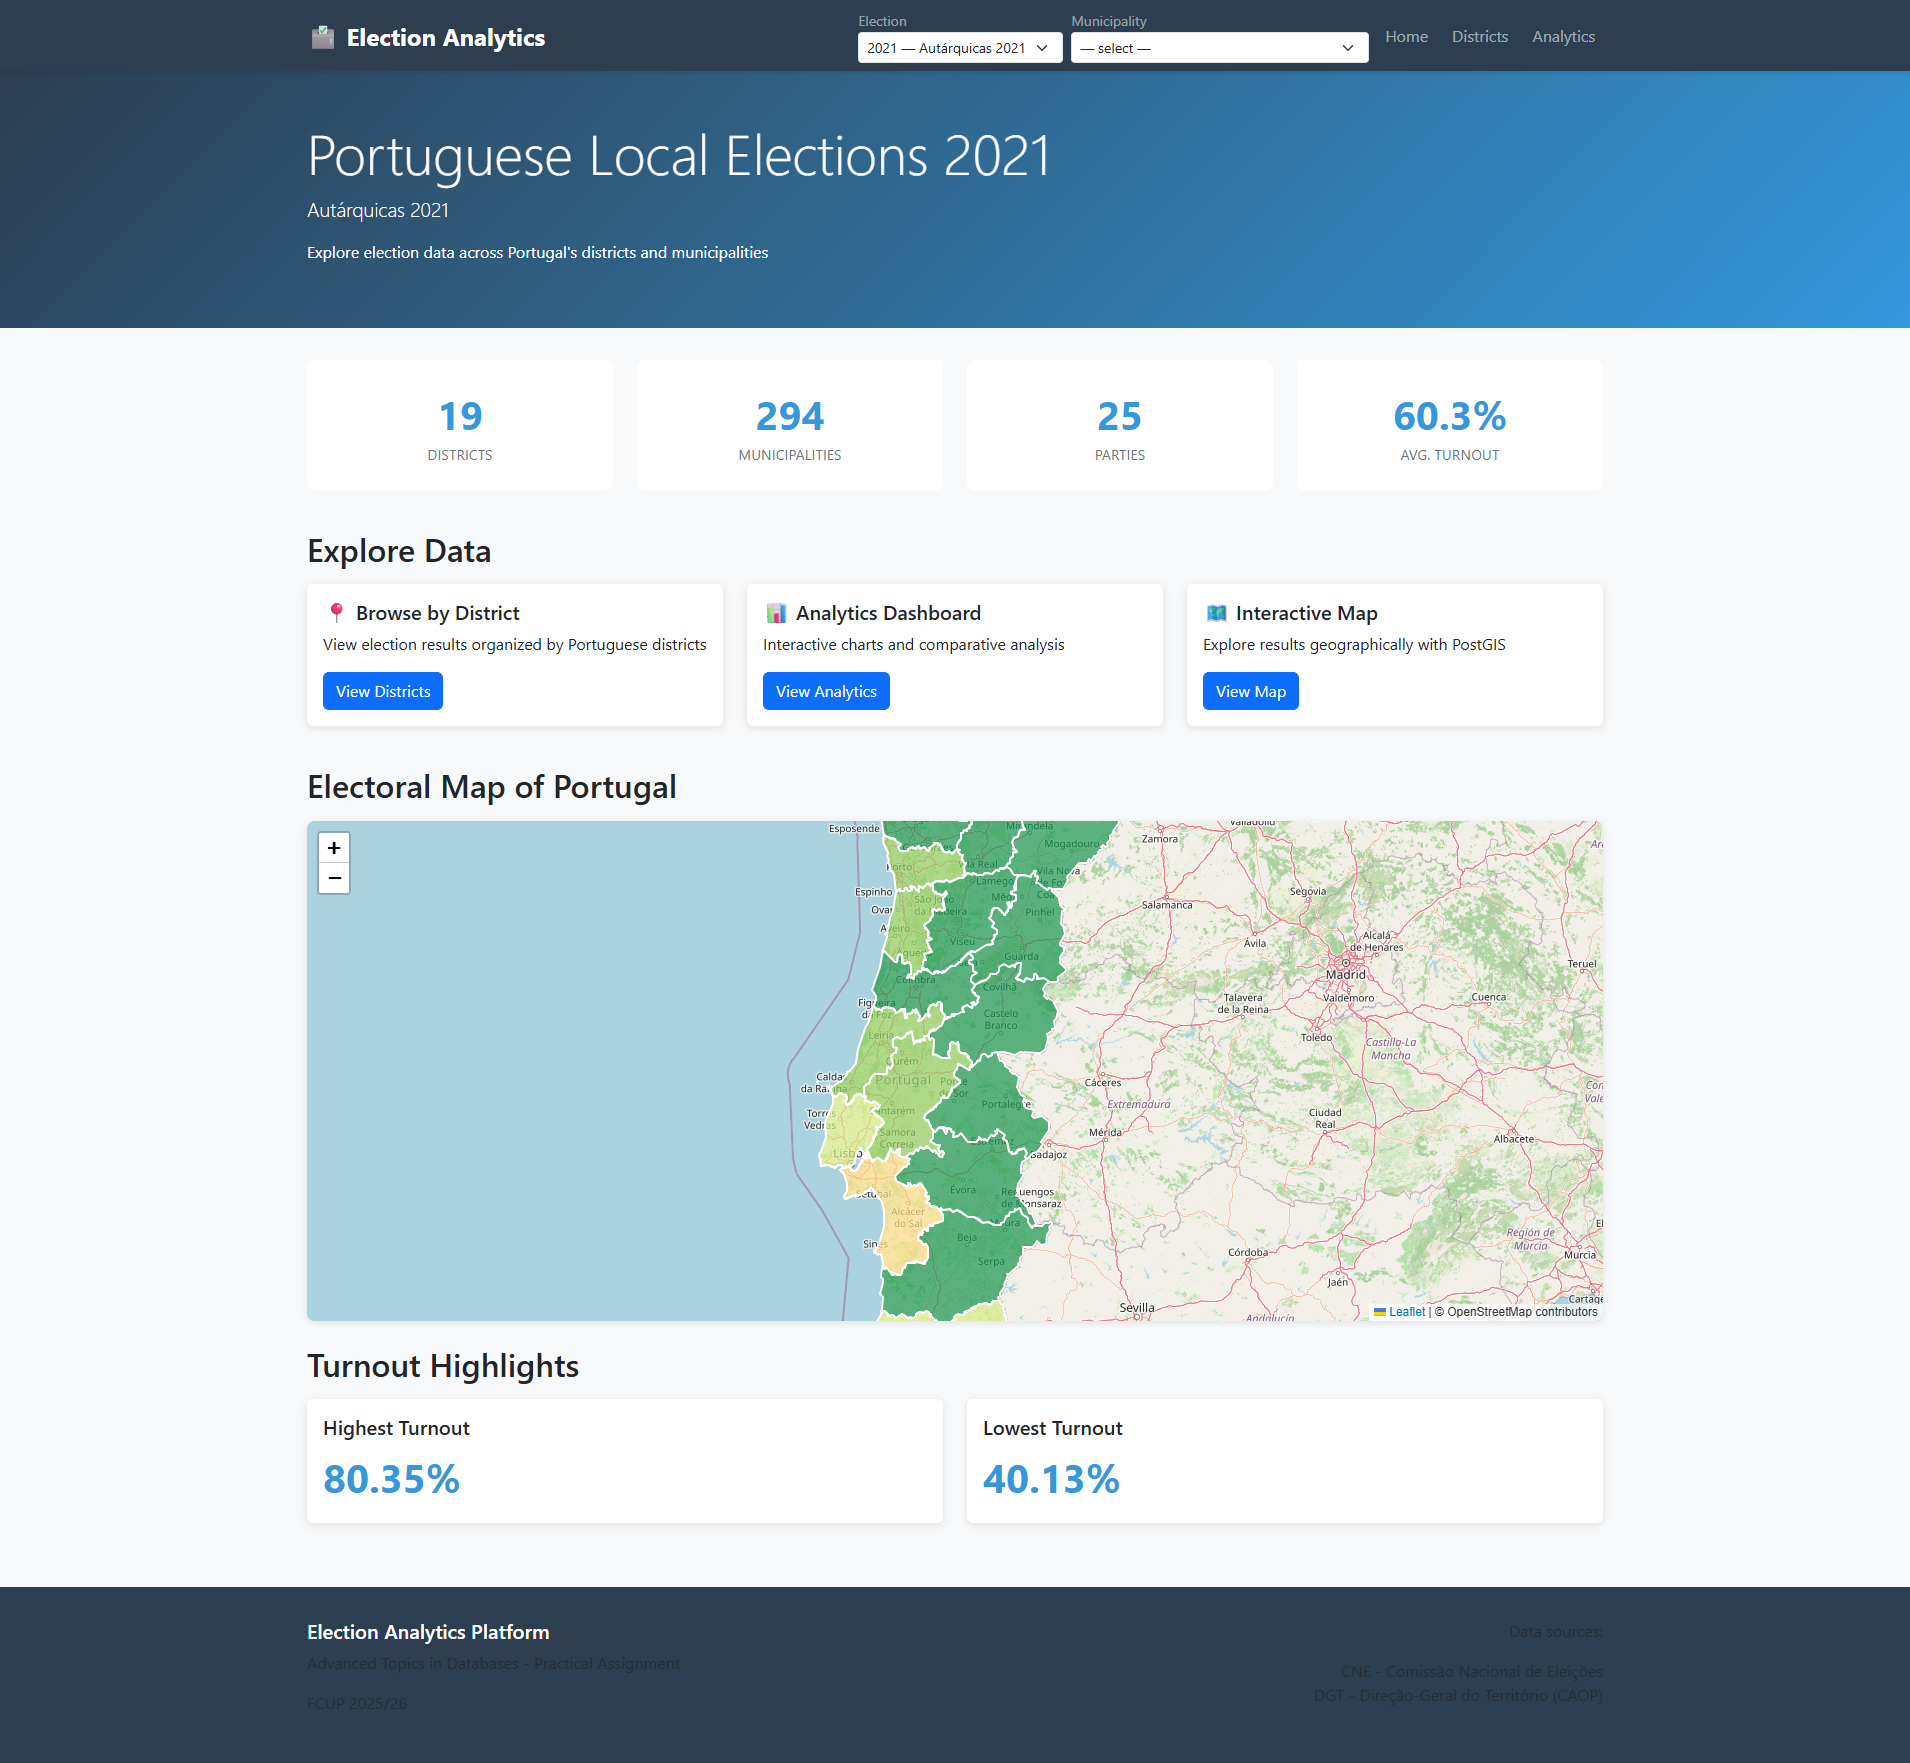
\includegraphics[width=0.92\textwidth]{../screenshots/home.png}
    \caption{Home page: election selector, summary cards, Leaflet district map (PostGIS geometries), and turnout highlights.}
    \label{fig:home}
\end{figure}

\begin{figure}[htbp]
    \centering
    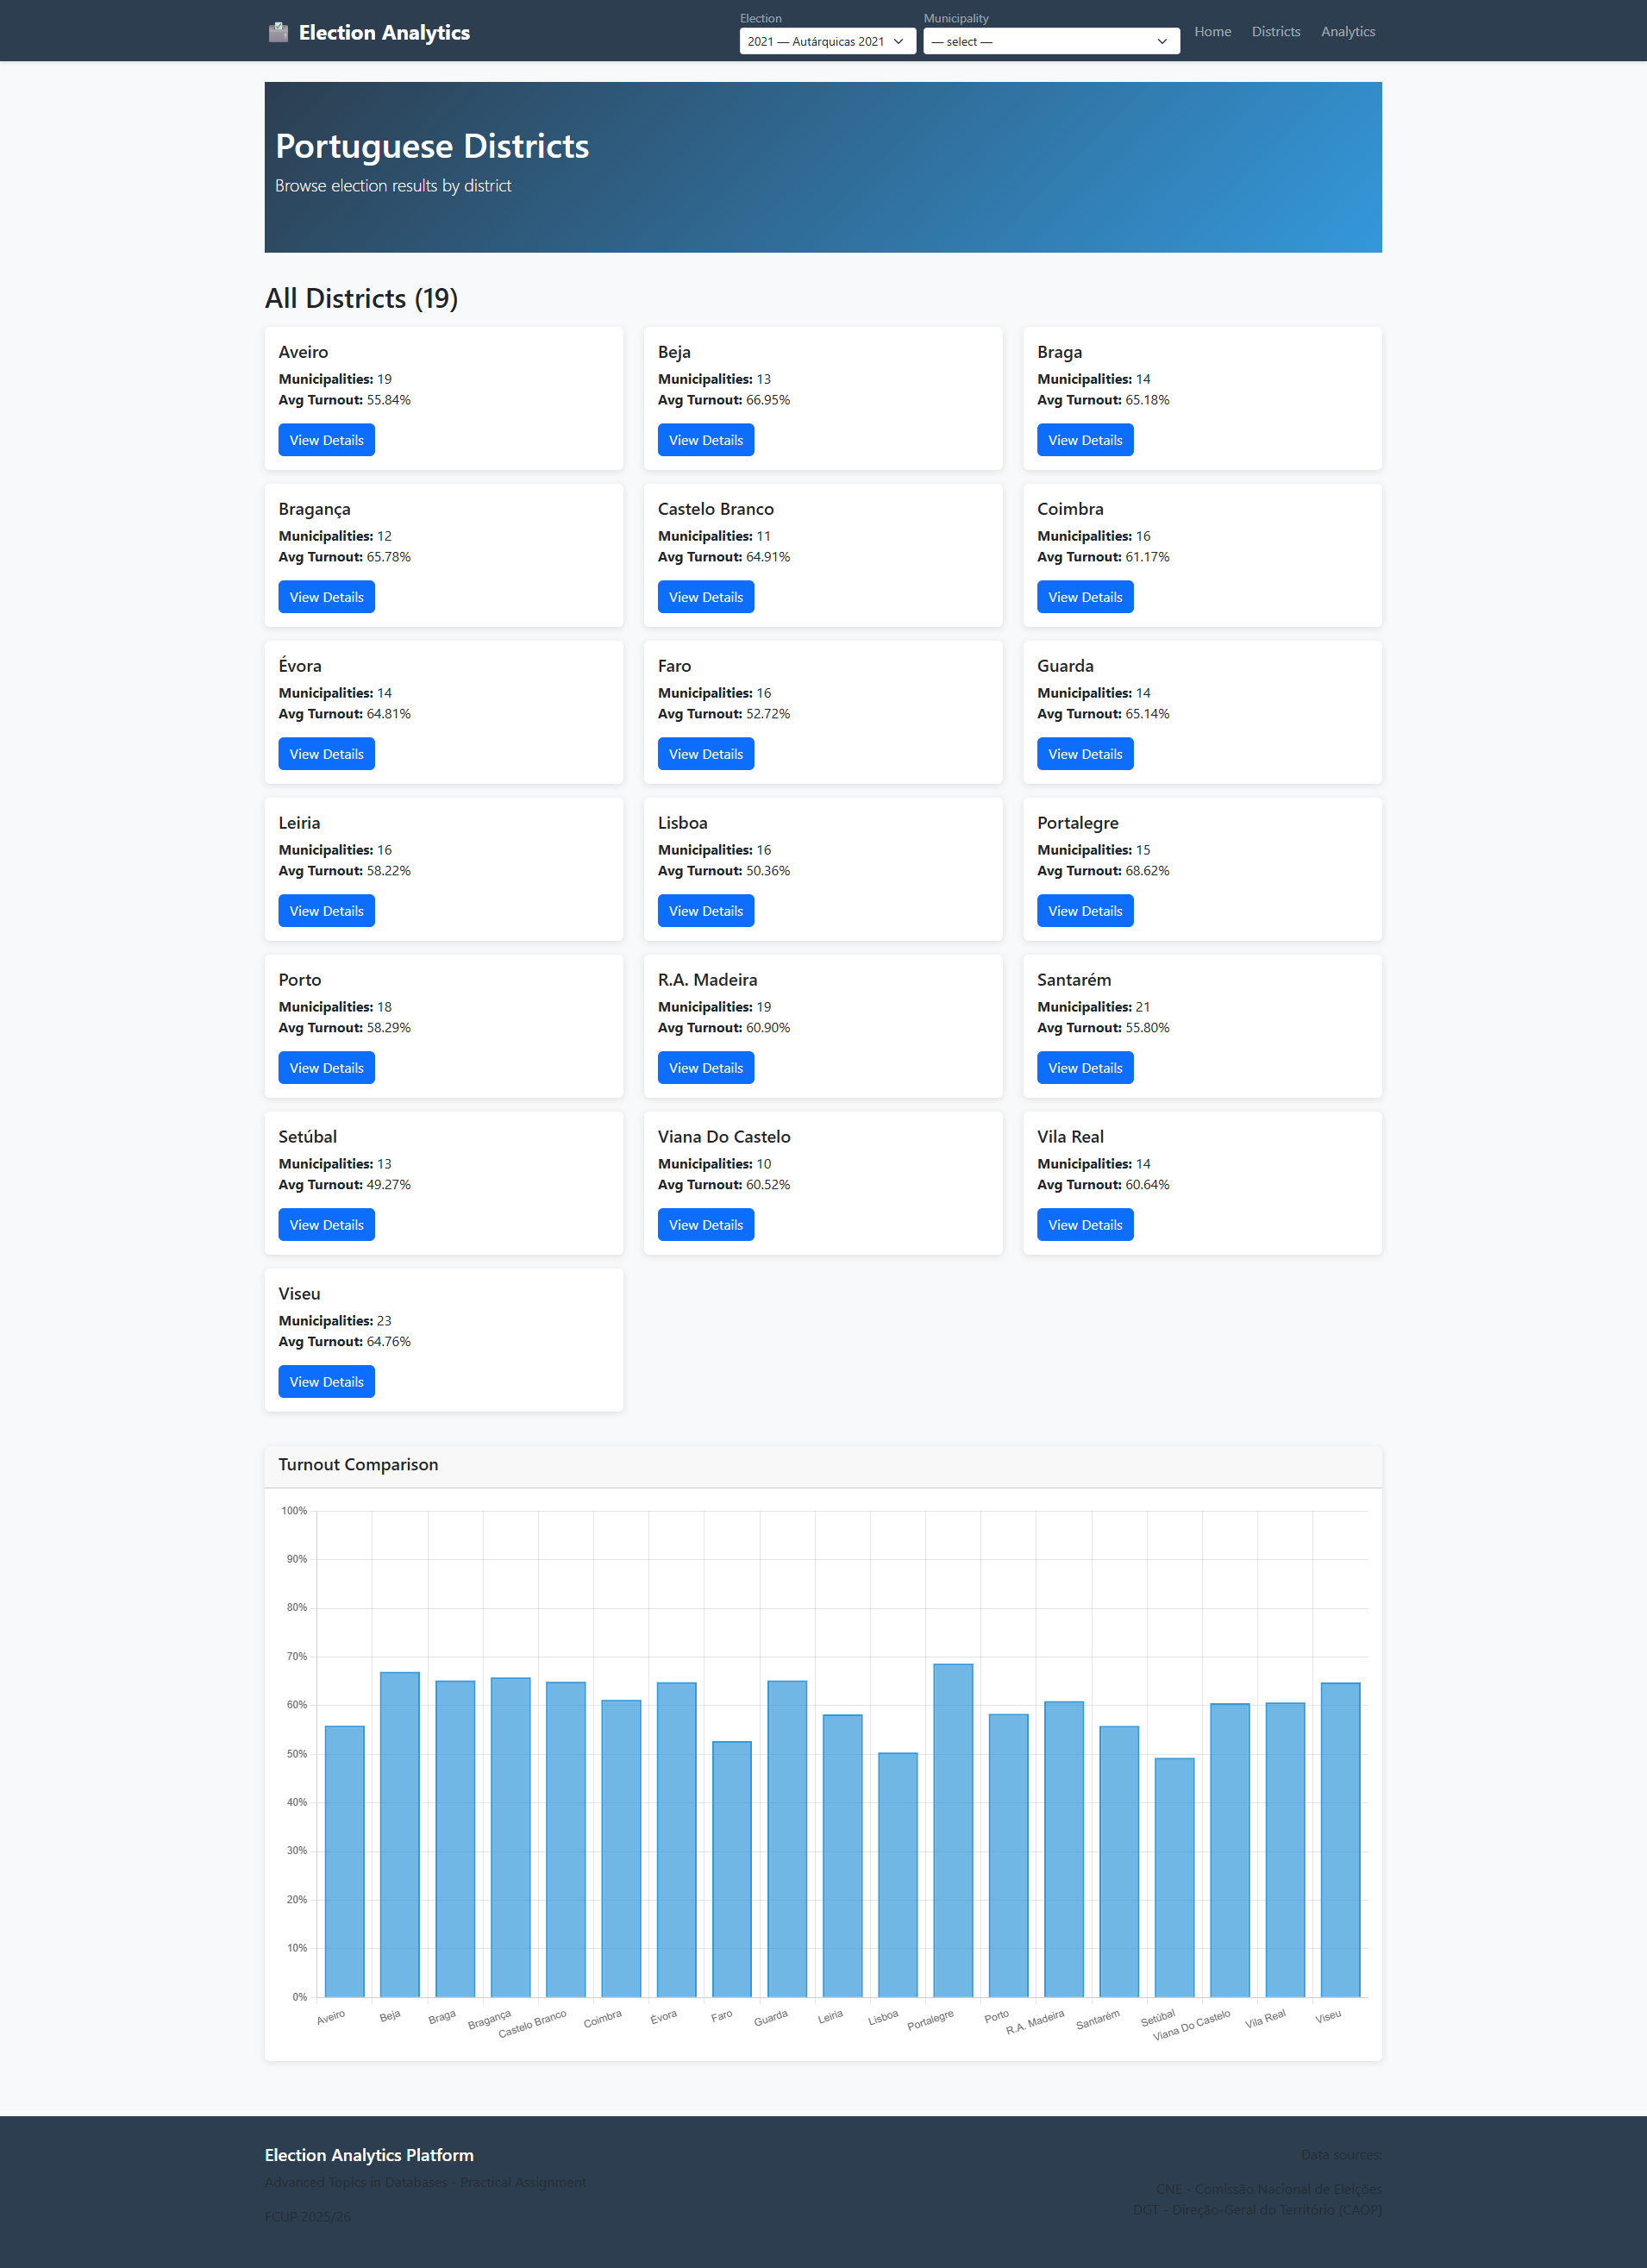
\includegraphics[width=0.92\textwidth]{../screenshots/districts.png}
    \caption{Districts page: per-district municipality counts and turnout, with Chart.js comparison across districts.}
    \label{fig:districts}
\end{figure}

\begin{figure}[htbp]
    \centering
    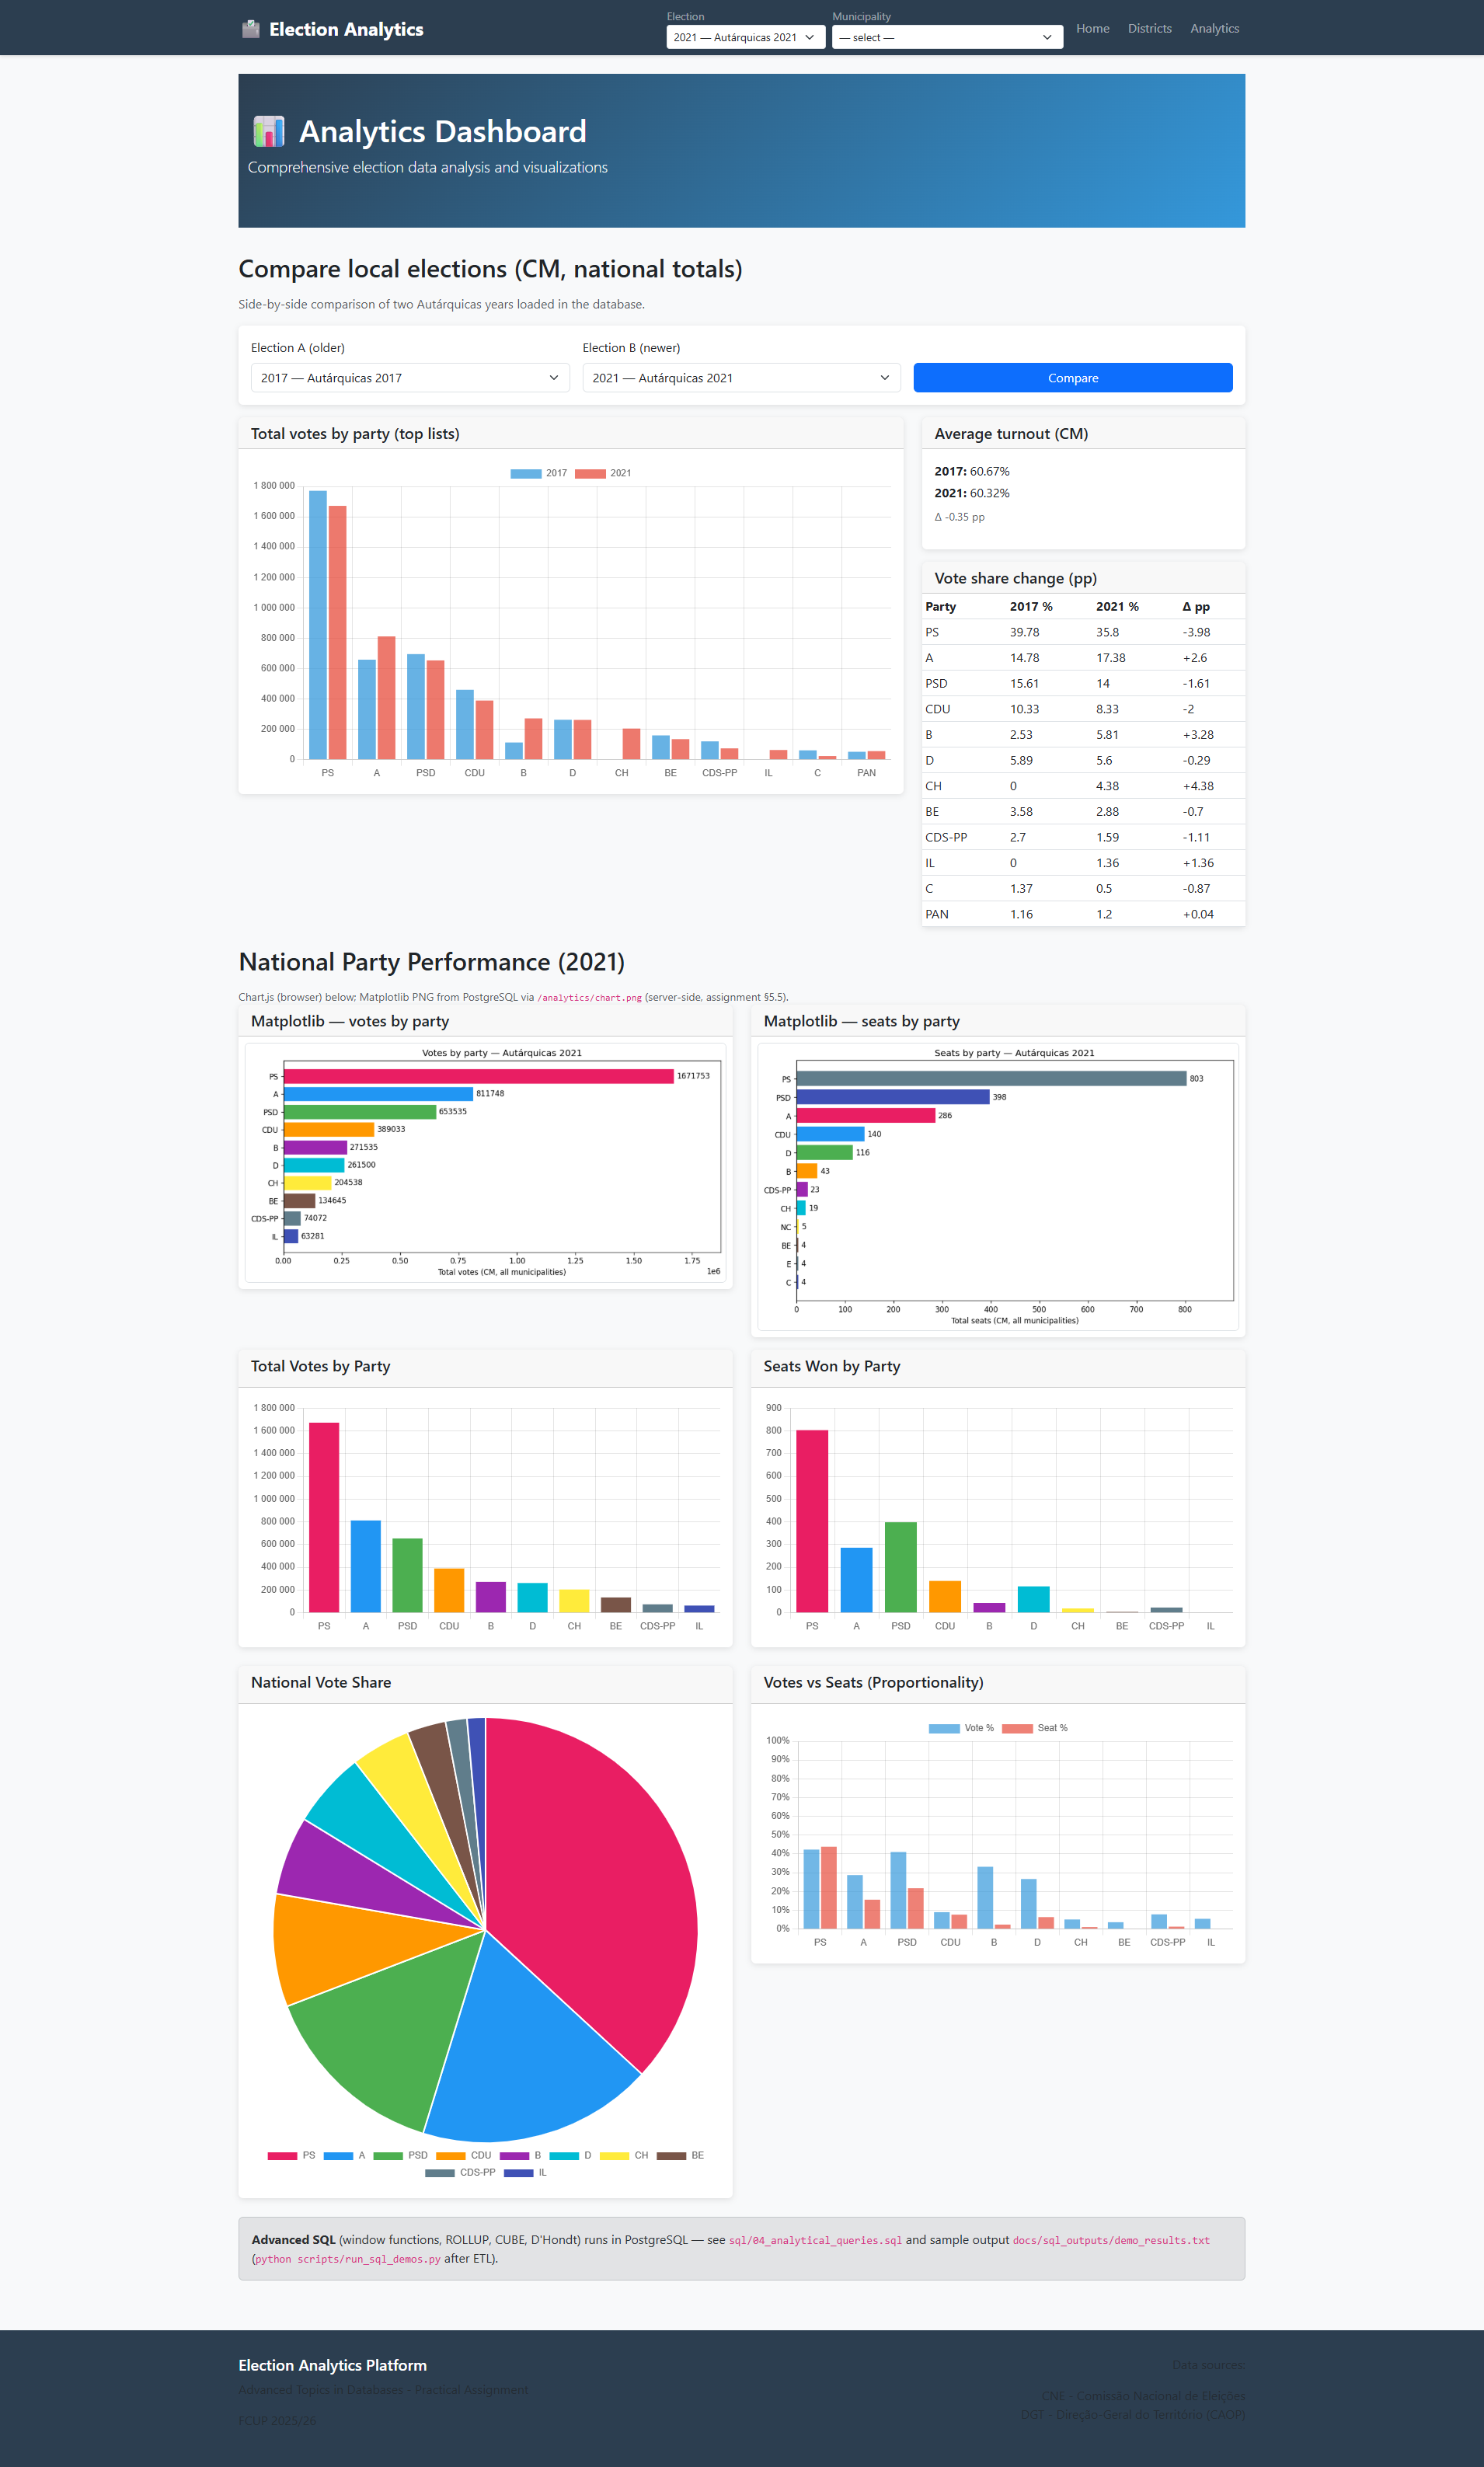
\includegraphics[width=0.92\textwidth,height=0.52\textheight,keepaspectratio]{../screenshots/analytics.png}
    \caption{Analytics dashboard: 2017 vs 2021 comparison, Matplotlib charts from PostgreSQL, and Chart.js vote/seat visualisations.}
    \label{fig:analytics}
\end{figure}

The UI deliberately uses operational/warehouse views and tailored API queries rather than the \texttt{analytical\_query\_*} views (see previous subsection). Run locally with \texttt{python app/app.py} on port 8000 after ETL (\texttt{docs/reproducibility.md}).

\subsection{Known Limitations and Possible Extensions}
\textbf{Current scope and gaps.}
\begin{itemize}
    \item \textbf{Elections and organ:} only Autárquicas \textbf{2017} and \textbf{2021}, organ \textbf{Câmara Municipal (CM)}, \textbf{municipality} level. Not loaded: \texttt{mapa\_3} (elected persons), Assembleia Municipal, Junta de Freguesia, or parish-level facts (parish exists in DDL only).
    \item \textbf{Party identity:} lists use \textbf{local codes} (e.g.\ A/B in Lisboa 2021); cross-year or national party comparison is misleading without manual mapping.
    \item \textbf{Source gaps:} $\sim$50 municipalities appear in CNE \texttt{mapa\_2} without matching \texttt{mapa\_1} rows, so they have seat metadata but no vote facts in the database.
    \item \textbf{Geography:} CAOP fallback GeoJSON covers the \textbf{continent}; island municipalities may lack \texttt{geometry} until full official shapefiles are added.
    \item \textbf{Warehouse:} tables \texttt{warehouse.agg\_*} are defined but \textbf{not populated} in the MVP pipeline.
    \item \textbf{Operations:} no user authentication; ETL is \textbf{batch} only (not live election-night ingestion). Turnout percentages require post-load refresh on older runs (\texttt{post\_load.py} or \texttt{scripts/fix\_turnout\_percentages.py}) because bulk load disables triggers.
    \item \textbf{Web vs SQL:} advanced \texttt{analytical\_query\_*} views are not exposed in the Flask UI (see Analytical Queries).
\end{itemize}

\textbf{Possible extensions.}
\begin{itemize}
    \item Populate \texttt{agg\_*}, add AM/JF organs and parish-level ETL; load additional election years into \texttt{DATASETS}.
    \item Full CAOP (including islands); richer map UX (e.g.\ AJAX detail panel) or Plotly dashboards.
    \item Wire selected analytical views into dedicated report/export pages; national-party normalization table for cross-municipality comparison.
\end{itemize}
\subsection{Short Statement of Individual Contributions}

\noindent\textbf{Amos Uwamusi up202502075}

\noindent Designed the \textbf{operational, staging, and warehouse database schemas}; implemented \textbf{SQL functions, triggers, and analytical queries} including D'Hondt allocation; built the first version of the \textbf{Flask web application} and page templates; developed the \textbf{initial ETL pipeline} and core project documentation; corrected analytical query definitions after testing.

\medskip
\noindent\textbf{Kamil Tasarz up202512958}

\noindent Refactored the ETL into \textbf{modular pipeline stages} and full-load orchestration; added loading of \textbf{official seat results} and \textbf{Aut\'{a}rquicas 2017} data for cross-year use; performed \textbf{CNE validation} and wrote reconciliation and reproducibility documentation; exported \textbf{ER diagrams} and prepared SQL demonstration outputs for the report; extended the web application with \textbf{analytics charts} and cross-election comparison APIs; fixed data-quality issues in turnout, seats, and charts; consolidated the project README and task list.

\medskip
\noindent\textbf{S\'{e}rgio Cardoso up202107918}

\noindent Obtained and organised \textbf{CNE election datasets} and Python dependencies for the team; contributed to early ETL configuration and schema setup alongside the data files; authored and maintained the \textbf{LaTeX final report} and \textbf{Beamer presentation slides}; updated report and slide content as the implementation evolved.